\chapter{Desarrollo Experimental}
\label{chap:desarrollo}

En este capítulo se detallan los procedimientos instrumentales y los desarrollos analíticos para cada una
de las experiencias llevadas a cabo en el laboratorio. Los datos experimentales obtenidos se vuelcan
en sus correspondientes tablas acompañados del análisis de incertidumbre pertinente.

El trabajo práctico se divide en dos partes diferenciadas según el amplificador bajo ensayo:
\begin{itemize}
    \item \textbf{Primera Parte (Experimentos 1 al 4):} Se trabaja sobre un amplificador de baja frecuencia.
    \item \textbf{Segunda Parte (Experimentos 5 al 8):} Se trabaja con un amplificador de dos etapas en el cual se puede realimentar la entrada negativamente mediante un jumper.
\end{itemize}

\section{Experimento 1: Determinación de la impedancia de salida del amplificador}
Como se mencionó anteriormente, a partir de este primer experimento al experimento 4 se trabaja sobre el primer amplificador
(amplificador de baja frecuencia) que se puede observar en la figura
\ref{fig:amplificador_baja_frecuencia}.

\begin{figure}[!ht]
    \centering
    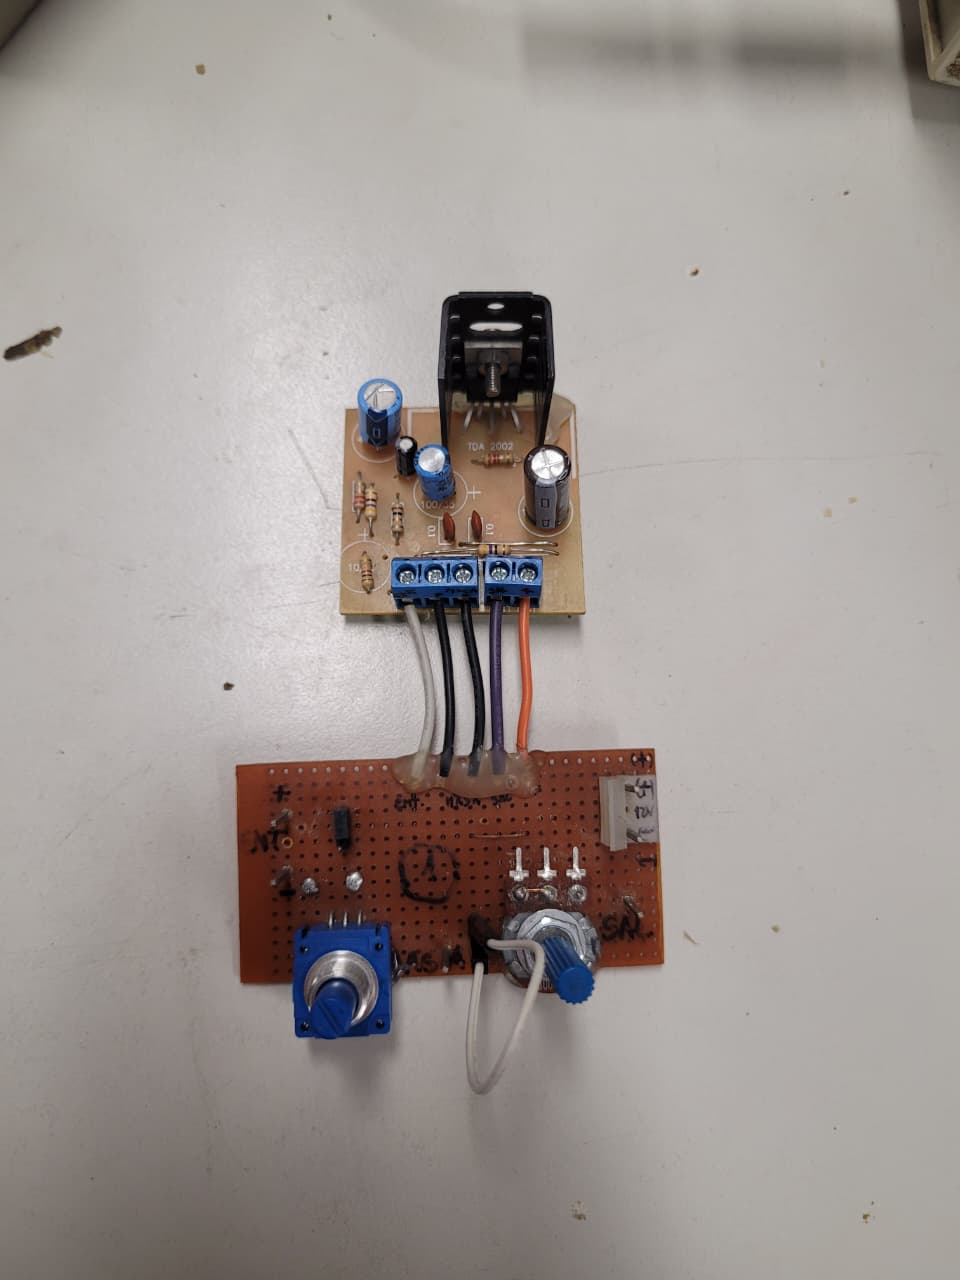
\includegraphics[width=0.4\textwidth]{images/amplificador_baja_frecuencia.jpeg}
    \caption{Amplificador de baja frecuencia.}
    \label{fig:amplificador_baja_frecuencia}
\end{figure}

El ensayo para medir la impedancia de salida ($Z_o = R_o$) se basa en el método de sustitución y reducción a
la mitad de la tensión sobre una carga conocida. Se conectó el instrumental según el esquema de la
Figura~\ref{fig:crkt_medicion_ro}.

\begin{figure}[!ht]
    \centering
    % Aquí se puede incluir el gráfico tikz o la captura del circuito
    \resizebox{\textwidth}{!}{%
        \begin{tikzpicture}[transform shape]
	% Paths, nodes and wires:
	\node[shape=rectangle, draw, line width=1pt, minimum width=4.965cm, minimum height=2.965cm] at (9.5, 1.5){};
	\node[shape=rectangle, draw, line width=1pt, minimum width=2.215cm, minimum height=1.465cm] at (10.375, 1.75){};
	\node[shape=rectangle, draw, line width=1pt, minimum width=3.965cm, minimum height=2.965cm] at (-0, 1.5){} node[anchor=center, align=center, text width=3.577cm, inner sep=6pt] at (-0, 1.5){Amplificador};
	\node[shape=rectangle, draw, line width=1pt, minimum width=3.965cm, minimum height=2.965cm] at (-9, 1.5){};
	\draw (-5.61, 1.5) to[bare jumper, l_={$J_2$}] (-5.61, 0.5);
	\draw (-5.61, 0.5) to[variable american resistor, l_={$R_{in}$}] (-3.36, 0.5);
	\draw (-5.61, 1.5) to[closed jumper, l={$J_1$}] (-5.61, 2.5);
	\draw (-7.36, 1.5) -| (-5.61, 1.5);
	\draw (-5.61, 2.5) -- (-3.36, 2.5) -| (-3.36, 1.5) -| (-2, 1.5);
	\draw (-3.36, 0.5) -| (-3.36, 1.5);
	\draw (3.5, 0.5) to[variable american resistor, l_={$R_{L}$}] (3.5, -2);
	\draw (3.5, 1.5) to[bare jumper, l_={$J_3$}] (3.5, 0.5);
	\draw (5.5, -2) to[voltmeter, mirror] (5.5, 0.5);
	\draw (2, 1.5) -| (3.5, 1.5) -- (5, 1.5) -| (7.61, 1.5);
	\draw (5.5, 0.5) -| (5.5, 1.5);
	\node[ground] at (-0, -2){};
	\node[ground] at (-7.5, -2){};
	\node[ground] at (3.5, -2){};
	\node[ground] at (5.5, -2){};
	\node[ground] at (7.75, -2){};
	\draw (7.75, -2) -- (7.75, 1.25);
	\draw (-7.5, -2) -- (-7.5, 1.25);
	\draw (-0, -2) -- (-0, -0);
	\draw (7.75, 1.75) to[currtap] (7.75, 1.25);
	\draw (-7.5, 1.75) to[currtap, mirror] (-7.5, 1.25);
	\node[shape=rectangle, minimum width=4.465cm, minimum height=0.715cm] at (-9, 3.375){} node[anchor=center, align=center, text width=4.077cm, inner sep=6pt] at (-9, 3.375){Generador de funciones};
	\node[shape=rectangle, minimum width=4.465cm, minimum height=0.715cm] at (9.5, 3.375){} node[anchor=center, align=center, text width=4.077cm, inner sep=6pt] at (9.5, 3.375){Osciloscopio};
\end{tikzpicture}%
    }
    \caption{Esquema de conexión de instrumentos para la medición de la impedancia de salida.}
    \label{fig:crkt_medicion_ro}
\end{figure}

El procedimiento consistió en los siguientes pasos:
\begin{enumerate}
    \item Con la resistencia de carga ($R_L$) desconectada (circuito abierto/vacío), se aplicó una señal
          senoidal de $1\kHz$ en la entrada, regulando la amplitud de salida para asegurar la máxima excursión
          simétrica sin distorsión por recorte. Se midió la tensión de salida
          $V_s = 10.6V_{pp}$.
    \item Se conectó la resistencia de carga variable $R_L$ mediante el jumper $J_1$ y se disminuyó su valor progresivamente
          desde el máximo hasta lograr que la tensión de salida se reduzca exactamente a la mitad de la
          medida en vacío ($V_s' = V_s / 2 = 5.3V_{pp}$).
    \item En esta condición de divisor resistivo, el valor óhmico de $R_L$ es numéricamente equivalente
          a la impedancia de salida ($R_o$). Se interrumpió la alimentación y se
          midió el valor de $R_L = 42\ohm$
          con el multímetro digital.
\end{enumerate}

Para determinar el error instrumental asociado a la
medición de la resistencia $R_L = R_o$, se consideraron las especificaciones
técnicas del fabricante del multímetro digital utilizado, el UNI-T UT33A+. El
manual de este instrumento indica que para el rango de $200\ohm$, posee una
precisión de $\pm(1.0\% + 2)$ dígitos con una resolución de $0.1\ohm$.

Dado que el valor medido fue de $42\ohm$ (comprendido en el rango de $200\ohm$), el cálculo de la incertidumbre absoluta de la medición ($\Delta R_L$) se desarrolla como:
\begin{equation}
    \Delta R_L = \pm \left( 1.0\% \cdot R_{\text{medido}} + 2 \cdot \text{resolución} \right)
\end{equation}
\begin{equation}
    \Delta R_L = \pm \left( 0.01 \cdot 42\ohm + 2 \cdot 0.1\ohm \right) = \pm \left( 0.42\ohm + 0.2\ohm \right) = \pm 0.62\ohm
\end{equation}

Expresando el resultado final con un decimal de acuerdo con la resolución del equipo, se obtiene una incertidumbre de $\pm 0.6\ohm$.

En la Figura~\ref{fig:medicion_ro_exp1} se presenta el registro fotográfico de la medición de esta resistencia con el multímetro digital en el laboratorio, donde se puede apreciar que el valor arrojado por el instrumento para la impedancia de salida es de $42\ohm$.

Los resultados del ensayo se resumen en la Tabla~\ref{tab:exp1}.

\begin{table}[!ht]
    \centering
    \begin{tabular}{|c|c|c|c|c|}
        \hline
        Frecuencia ($f_1$) & $Z_{sal}$ Nominal & $V_s$ (Vacío) & $R_L = R_o$ & Incertidumbre $R_L$ \\ \hline
        $1\kHz$ & $50\ohm$ & 10.6 $\V_{pp}$ & $42.0\ohm$ & $\pm 0.6\ohm$ \\ \hline
    \end{tabular}
    \caption{Resultados de la medición de la impedancia de salida.}
    \label{tab:exp1}
\end{table}

\begin{figure}[!ht]
    \centering
    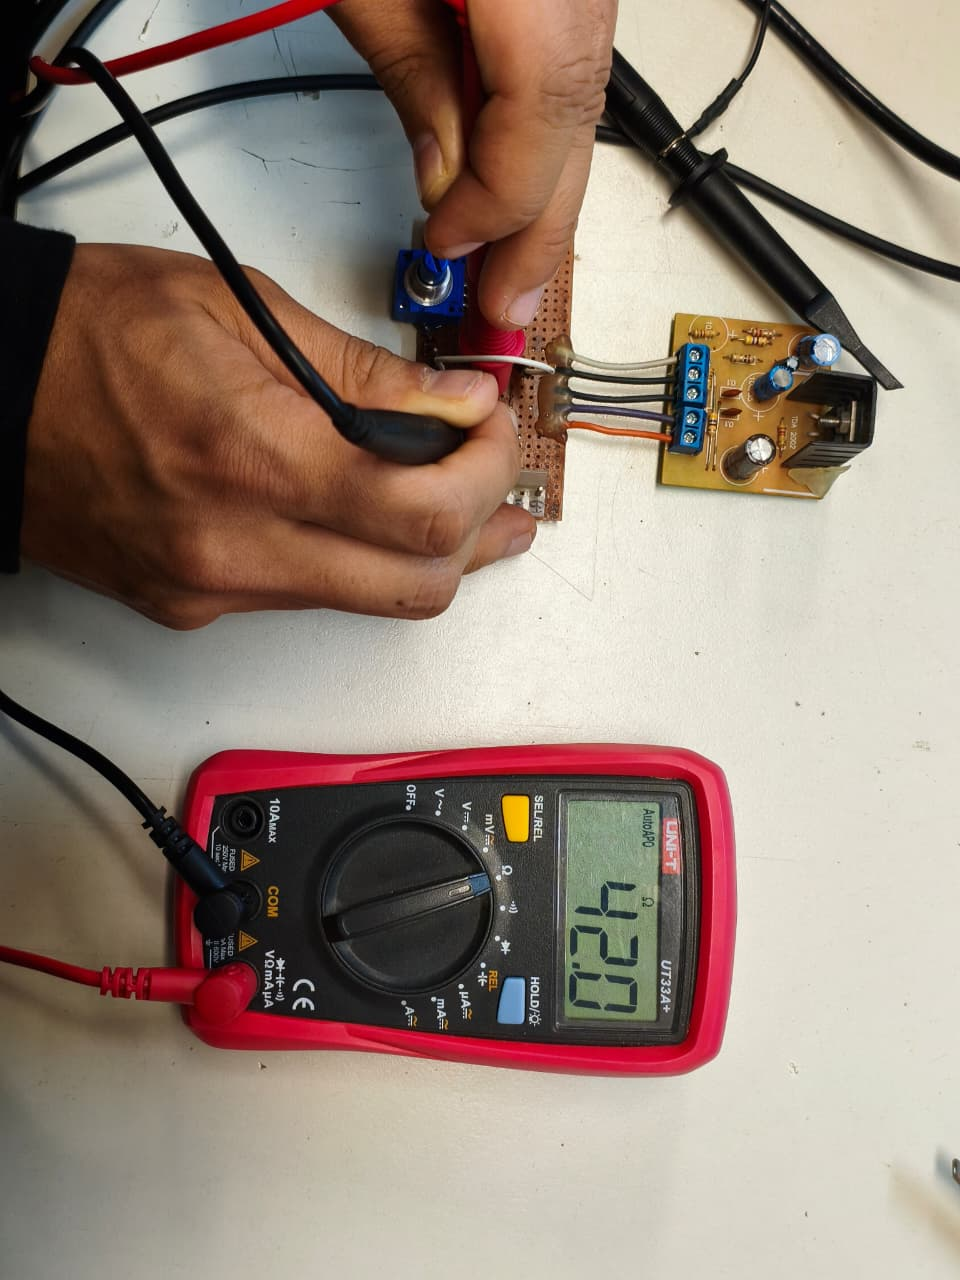
\includegraphics[width=0.4\textwidth,angle=90]{images/medicion_ro_exp1.jpeg}
    \caption{Medición de la impedancia de salida.}
    \label{fig:medicion_ro_exp1}
\end{figure}

\section{Experimento 2: Determinación de la impedancia de entrada del amplificador}
La medición de la impedancia de entrada ($Z_i = R_i$) se realizó colocando un
resistor variable ($R_{e1}$ que se se encuentra en la figura
\ref{fig:crkt_medicion_ro}) en la entrada del amplificador.

El procedimiento operativo fue:
\begin{enumerate}
    \item Con la entrada del amplificador conectada de forma directa ($R_{e1} = 0\ohm$), se excitó con una señal
          senoidal de $1\kHz$ y se ajustó para obtener una tensión de salida simétrica y libre de distorsión,
          registrando este valor inicial de tensión $V_s = 10.6V_{pp}$.
    \item Se intercaló la resistencia variable de entrada ($R_{e1}$) inicialmente en su valor mínimo, y se
          incrementó gradualmente hasta que la tensión medida en la salida cayó a la mitad de su valor inicial
          ($V_s' = V_s/2 = 5.3V_{pp}$).
    \item Bajo esta condición, la caída de tensión en el resistor variable es igual a la tensión 
          sobre la impedancia de entrada del amplificador, lo que implica que
          $R_{e1} = R_i$. El valor medido con el multímetro fue de $R_{e1} = 1096\ohm$.
\end{enumerate}

Para determinar el error instrumental asociado a la medición de la resistencia $R_{e1} = R_i$, se consideraron las especificaciones técnicas del fabricante del multímetro digital en el rango de $2000\ohm$, el cual posee una precisión de $\pm(0.7\% + 2)$ dígitos con una resolución de $1\ohm$.

Dado que el valor medido fue de $1096\ohm$, el cálculo de la incertidumbre absoluta de la medición ($\Delta R_{e1}$) se desarrolla como:
\begin{equation}
    \Delta R_{e1} = \pm \left( 0.7\% \cdot R_{e1} + 2 \cdot \text{resolución} \right)
\end{equation}
\begin{equation}
    \Delta R_{e1} = \pm \left( 0.007 \cdot 1096\ohm + 2 \cdot 1\ohm \right) = \pm \left( 7.672\ohm + 2\ohm \right) = \pm 9.672\ohm
\end{equation}

Expresando el resultado final sin decimales de acuerdo con la resolución de $1\ohm$ de la escala del instrumento, se obtiene una incertidumbre de $\pm 10\ohm$.

Los valores relevados en la práctica se indican en la Tabla~\ref{tab:exp2}.

\begin{table}[!ht]
    \centering
    \begin{tabular}{|c|c|c|c|c|}
        \hline
        Frecuencia ($f_1$) & $Z_{ent}$ Nominal & $V_s$ (Directo) & $R_{e1} = R_i$ & Incertidumbre $R_{e1}$ \\ \hline
        $1\kHz$ & $1000\ohm$ & 10.6 $\V_{pp}$ & 1096 $\ohm$ & $\pm 10\ohm$ \\ \hline
    \end{tabular}
    \caption{Resultados de la medición de la impedancia de entrada.}
    \label{tab:exp2}
\end{table}

\section{Experimento 3: Medición de la potencia de salida del amplificador}
La potencia de salida se determinó sobre una carga adaptada al valor de impedancia de salida medida en el
Experimento 1 ($R_L = R_o = 42\ohm$). La medición de tensión se realizó mediante un multímetro analógico
\textit{UNIVO} con escala en decibeles ($dB$), resultando en valor de
$V_{sal}=7.2dBu$, como se observa en la figura \ref{fig:exp4_salida_dbu}.

\begin{figure}[!ht]
    \centering
    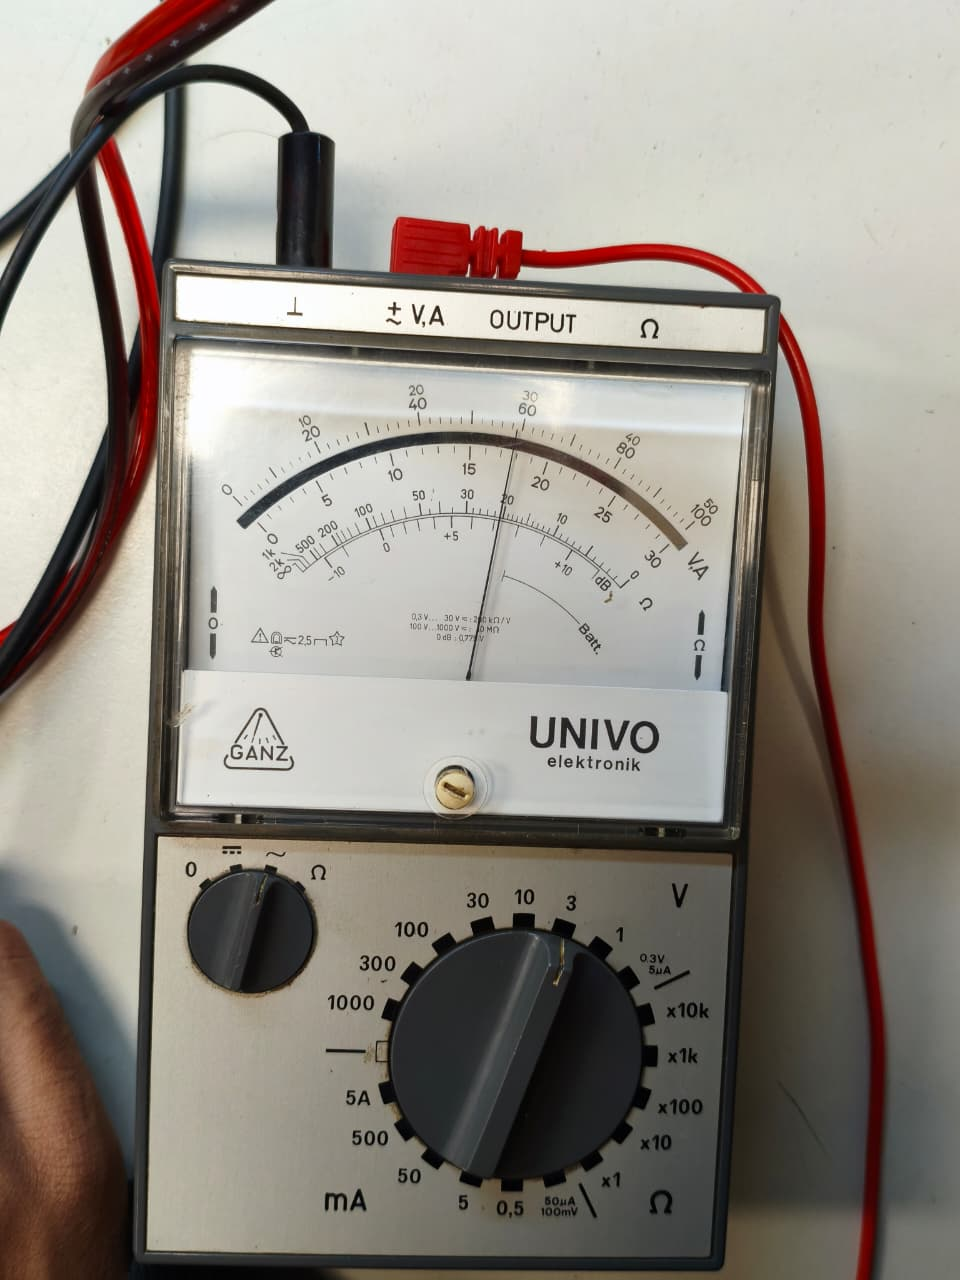
\includegraphics[width=0.5\textwidth]{images/exp_4_med_pot_sal_db.jpeg}
    \caption{Medición tensión de salida en dBu.}
    \label{fig:exp4_salida_dbu}
\end{figure}

Dado que la escala del multímetro analógico está calibrada para mediciones de tensión de CA sobre cargas de referencia
de $600\ohm$ (donde $0\dBu \equiv 0,775\V$), se aplicó la fórmula de corrección para obtener la potencia real
expresada en $dBm$ sobre la impedancia medida $R_o$:
\begin{equation}
    P_{sal} [dBm] = V_{sal} [dBu] + 10 \cdot \log_{10} \left( \frac{600\ohm}{R_o} \right)
\end{equation}

Una vez calculado el nivel en $dBm$, la potencia eficaz expresada en watts se obtiene a partir de:
\begin{equation}
    P_{x} [\W] = 1\mW \cdot 10^{\frac{P_{sal} [dBm]}{10}}
\end{equation}

Los resultados y parámetros determinados para la máxima excursión simétrica se consignan en la Tabla~\ref{tab:exp3}.

\begin{table}[!ht]
    \centering
    \resizebox{\textwidth}{!}{
    \begin{tabular}{|c|c|c|c|c|}
        \hline
        \textbf{Carga Ajustada $R_o$} & \textbf{Lectura $V_{sal}$ [dBu]} & \textbf{Término Corrector [dB]} & \textbf{Potencia $P_{sal}$ [dBm]} & \textbf{Potencia $P_x$ [mW]} \\ \hline
        $42.0\ohm$ & $7.2\dBu$ & $11.55\dB$ & $18.75\dBm$ & $74.97\mW$ \\ \hline
    \end{tabular}}
    \caption{Determinación de la potencia de salida en carga adaptada utilizando escala en dB.}
    \label{tab:exp3}
\end{table}

\section{Experimento 4: Medición de la ganancia de tensión y ganancia de
potencia del amplificador} Para determinar la ganancia del amplificador se
midieron las señales de entrada y salida utilizando el mismo voltímetro de CA
(escala de decibeles $\dBu$). En este ensayo se utilizó la misma resistencia de
carga en la salida que en el experimento anterior ($R_l = R_o = 42\ohm$), por lo
que la tensión de salida $V_{sal} = 7.2\dBu$ y la potencia de salida corregida
$P_{sal} = 18.75\dBm$ son idénticas a las del Experimento 3. La señal de entrada
medida fue de $V_{ent} = -1.0\dBu$, como se observa en la imagen
\ref{fig:exp4_ent_db}.

\begin{figure}[!ht]
    \centering
    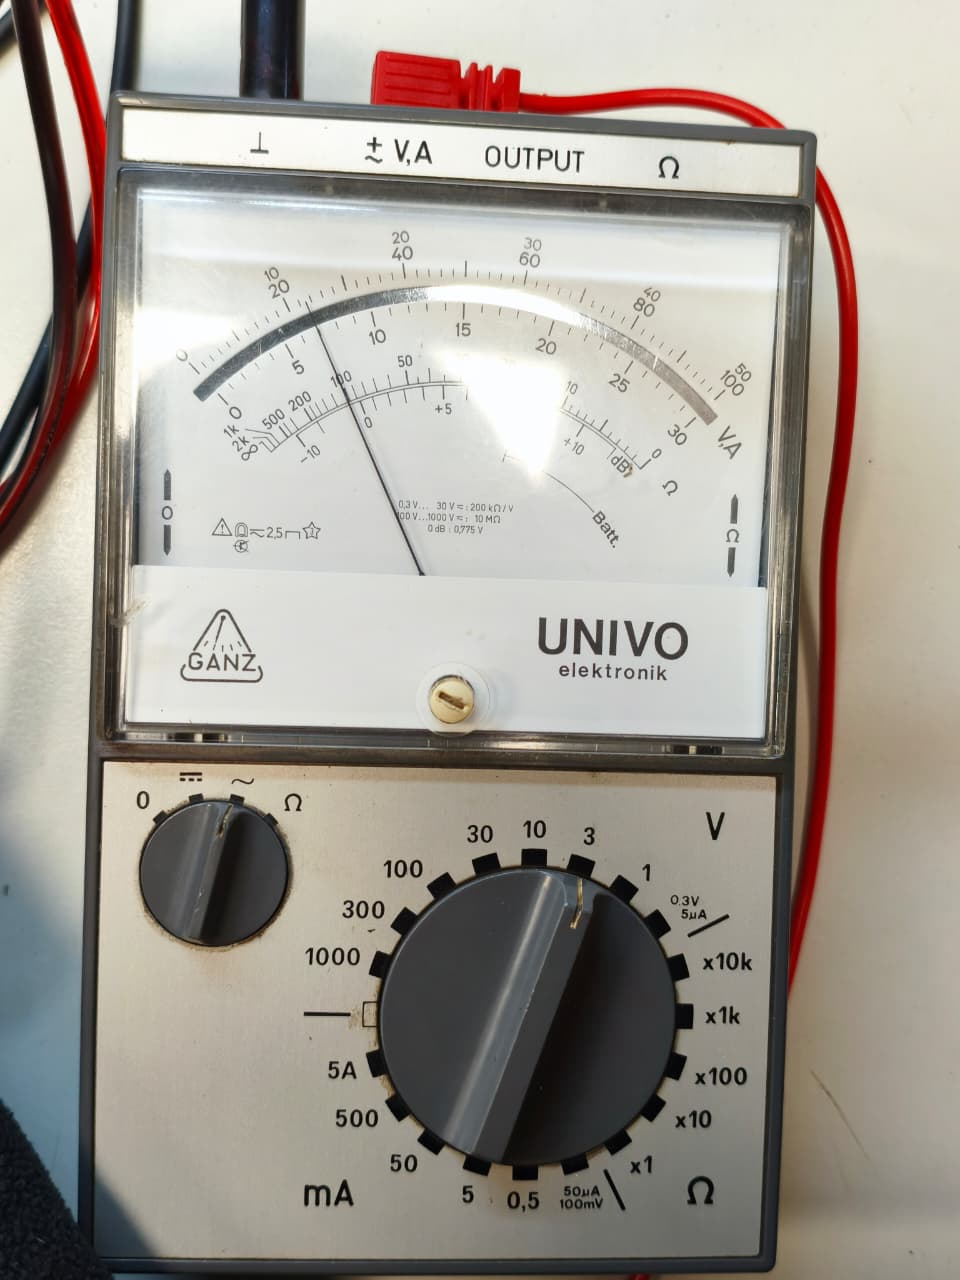
\includegraphics[width=0.5\textwidth]{images/exp_4_med_pot_ent_db.jpeg}
    \caption{Medición tensión de salida en dBu.}
    \label{fig:exp4_ent_db}
\end{figure}


La ganancia de tensión en $\dB$ se calcula directamente restando los niveles medidos en $\dBu$:
\begin{equation}
    A_v [\dB] = V_{sal} [\dBu] - V_{ent} [\dBu]
\end{equation}
Reemplazando por los valores experimentales:
\begin{equation}
    A_v [\dB] = 7.2\dBu - (-1.0\dBu) = 8.2\dB
\end{equation}
Expresando esta ganancia en veces (relación de tensión):
\begin{equation}
    A_v [\text{veces}] = 10^{\frac{A_v [\text{dB}]}{20}} = 10^{\frac{8.2}{20}} \approx 2.57\ \text{veces}
\end{equation}

Para calcular la ganancia de potencia, primero se determinan las potencias absolutas corregidas a $\dBm$ para la entrada ($P_{ent}$) y para la salida ($P_{sal}$):
\begin{equation}
    P_{ent} [\dBm] = V_{ent} [\dBu] + 10 \cdot \log_{10} \left( \frac{600\ohm}{R_i} \right)
\end{equation}
\begin{equation}
    P_{sal} [\dBm] = V_{sal} [\dBu] + 10 \cdot \log_{10} \left( \frac{600\ohm}{R_o} \right)
\end{equation}

Reemplazando los valores en la ecuación de potencia de entrada, considerando
la $R_i=1096\ohm$ del amplificador determinada en el Experimento 2:
\begin{equation}
    P_{ent} [\dBm] = -1.0\dBu + 10 \cdot \log_{10} \left( \frac{600\ohm}{1096\ohm} \right) = -1.0 - 2.62\dB = -3.62\dBm
\end{equation}
Mientras que para la potencia de salida se obtiene la misma ecuación y valor que en el Experimento 3:
\begin{equation}
    P_{sal} [\dBm] = 7.2\dBu + 10 \cdot \log_{10} \left( \frac{600\ohm}{42\ohm} \right) = 7.2 + 11.55\dB = 18.75\dBm
\end{equation}

La ganancia de potencia final en $\dB$ se obtiene como la diferencia de las potencias absolutas en $\dBm$:
\begin{equation}
    A_p [\dB] = P_{sal} [\dBm] - P_{ent} [\dBm]
\end{equation}
Sustituyendo los valores calculados:
\begin{equation}
    A_p [\dB] = 18.75\dBm - (-3.62\dBm) = 22.37\dB
\end{equation}
Expresando esta ganancia en veces (relación de potencia):
\begin{equation}
    A_p [\text{veces}] = 10^{\frac{A_p [\text{dB}]}{10}} = 10^{\frac{22.37}{10}} \approx 172.4\ \text{veces}
\end{equation}

Para estimar la incertidumbre en la medición de tensión expresada en decibeles
($\dBu$) se calcula la tensión eficaz ($V_{\text{ef}}$) correspondiente en
voltios a partir del valor en decibeles ($V_{\dBu}$) mediante la relación:

\begin{equation}
    V_{\text{ef}} = 0.775\V \cdot 10^{\frac{V_{\dBu}}{20}}
\end{equation}

Considerando la precisión del multímetro digital ($\pm 2.5\%$ de la lectura en
todos los rangos, según el manual digital del instrumento disponible en el pañol del laboratorio central), se determinan los límites de tensión por exceso ($V_{\text{max}}$) y por defecto ($V_{\text{min}}$):
\begin{equation}
    V_{\text{max}} = V_{\text{ef}} \cdot (1 + 0.025) \quad \text{y} \quad V_{\text{min}} = V_{\text{ef}} \cdot (1 - 0.025)
\end{equation}

Finalmente, estos límites se reconvierten a decibeles para observar su desviación respecto al valor nominal:
\begin{equation}
    V_{\text{max}} [\dBu] = 20 \cdot \log_{10} \left( \frac{V_{\text{max}}}{0.775\V} \right) = V_{\dBu} + 20 \cdot \log_{10}(1.025) \approx V_{\dBu} + 0.214\dB
\end{equation}
\begin{equation}
    V_{\text{min}} [\dBu] = 20 \cdot \log_{10} \left( \frac{V_{\text{min}}}{0.775\V} \right) = V_{\dBu} + 20 \cdot \log_{10}(0.975) \approx V_{\dBu} - 0.220\dB
\end{equation}

Como se observa, independientemente del valor nominal de tensión medido ($V_{\dBu}$), la precisión del instrumento de $\pm 2.5\%$ se traduce en una desviación de $+0.214\dB$ y $-0.220\dB$. Para fines prácticos de presentación, este intervalo asimétrico se simplifica reportando una incertidumbre absoluta de $\pm 0.22\dB$.

Los datos recabados en el ensayo junto con las conversiones a "veces" y las incertidumbres de medición se encuentran detallados en la Tabla~\ref{tab:exp4}.

\begin{table}[!ht]
    \centering
    \resizebox{\textwidth}{!}{
    \begin{tabular}{|c|c|c|c|c|c|}
        \hline
        \textbf{Frecuencia del} & \multirow{2}{*}{\textbf{Salida}} & \multirow{2}{*}{\textbf{Entrada}} & \textbf{Incertidumbre} & \textbf{Ganancia en dB} & \textbf{Ganancia en} \\
        \textbf{generador} & & & \textbf{medición de dBu} & \textbf{(Salida - Entrada)} & \textbf{``veces'' (Salida/Entrada)} \\ \hline
        \multirow{2}{*}{$1\kHz$} & $7.2\dBu$ & $-1.0\dBu$ & $\pm 0.22\dB$ & $A_v = 8.2\dB$ & $A_v = 2.57$ veces \\ \cline{2-6}
        & $18.75\dBm$ & $-3.62\dBm$ & $\pm 0.22\dB$ & $A_p = 22.37\dB$ & $A_p = 172.4$ veces \\ \hline
    \end{tabular}}
    \caption{Medición y cálculo de ganancia de tensión y potencia.}
    \label{tab:exp4}
\end{table}

\section{Experimento 5: Determinación de la Resistencia de salida a lazo abierto y a lazo cerrado}
Desde el experimento 5 hasta el 8 se trabajará con el segundo amplificador
(amplificador de dos etapas con realimentación negativa mediante jumper), el
cual se puede ver en la figura \ref{fig:amplificador_dos_etapas}.

\begin{figure}[!ht]
    \centering
    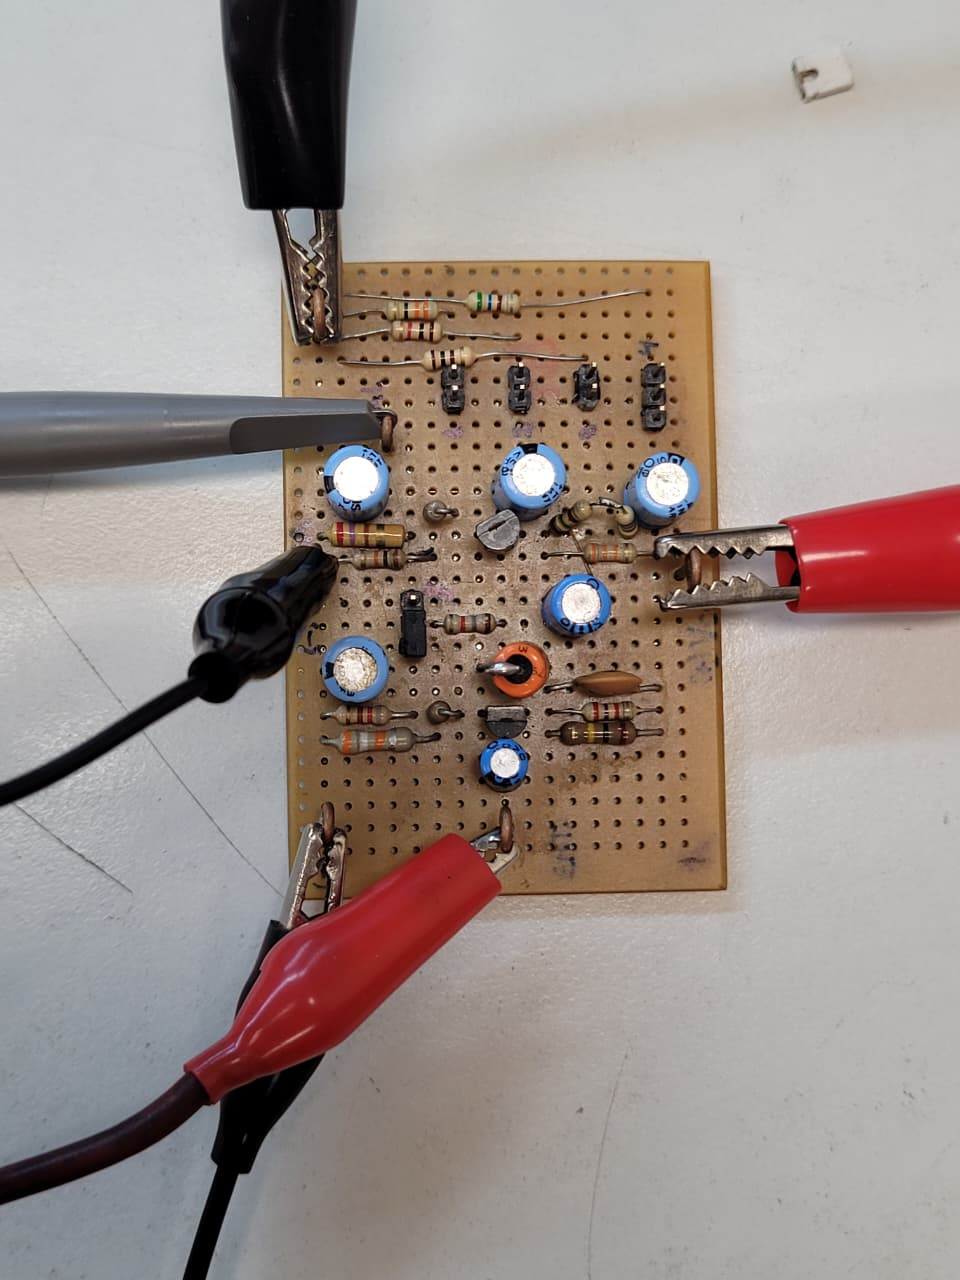
\includegraphics[width=0.5\textwidth, angle=90]{images/amplificador_dos_etapas.jpeg}
    \caption{Amplificador de dos etapas con jumper de realimentación.}
    \label{fig:amplificador_dos_etapas}
\end{figure}

Esta experiencia permite contrastar el comportamiento del amplificador bajo las
condiciones de lazo abierto (sin realimentación) y lazo cerrado (con
realimentación negativa de muestra de tensión y mezcla serie).

\subsection{Paso 1 y 2: Lazo Abierto (Sin realimentación)}
Con el jumper $J$ en posición abierta (sin realimentación) y a una frecuencia de excitación de $1\kHz$, se determinó:
\begin{itemize}
    \item La ganancia a lazo abierto ($A$) midiendo la entrada $V_i=42\mV_{pp}$ 
        y salida $V_{o,\text{vacío}}=7.2\V_{pp}$ ($Js$ desconectado) es de:
          \begin{equation}
              A = \frac{V_o}{V_i} = \frac{7.2\V_{pp}}{0.042\V_{pp}} \approx 171.43
          \end{equation}
    \item La resistencia de salida a lazo abierto ($R_o$) conectando la carga conocida $R_l = 1\kohm$ ($Js$ conectado)
        y registrando la tensión sobre la carga $V_s = 4.64V_{pp}$:
          \begin{equation}
              R_o = R_l \cdot \left( \frac{V_{o,\text{vacío}}}{V_s} - 1 \right) = 1000\ohm \cdot \left( \frac{7.2\V}{4.64\V} - 1 \right) = 1000\ohm \cdot \left( 1.5517 - 1 \right) \approx 551.7\ohm
          \end{equation}
\end{itemize}

\begin{figure}[!ht]
    \centering
    \begin{subfigure}[b]{0.48\textwidth}
        \centering
        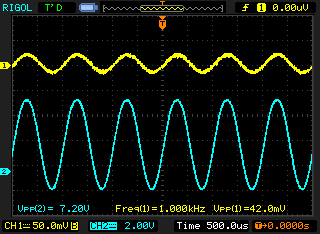
\includegraphics[width=\textwidth]{images/osc_exp5_vo_vacio.png}
        \caption{Tensión de salida en vacío ($V_{o,\text{vacío}} = 7.2\V_{pp}$).}
        \label{fig:osc_exp5_vo_vacio}
    \end{subfigure}
    \hfill
    \begin{subfigure}[b]{0.48\textwidth}
        \centering
        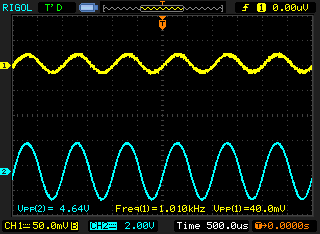
\includegraphics[width=\textwidth]{images/osc_exp5_vrl_1k.png}
        \caption{Tensión sobre la carga de $1\kohm$ ($V_s = 4.64\V_{pp}$).}
        \label{fig:osc_exp5_vrl_1k}
    \end{subfigure}
    \caption{Capturas de pantalla del osciloscopio en condición de lazo abierto.}
    \label{fig:osc_exp5_lazo_abierto_capturas}
\end{figure}

Los valores medidos y los resultados de los cálculos se resumen en la Tabla~\ref{tab:exp5_lazo_abierto}.

\begin{table}[!ht]
    \centering
    \resizebox{\textwidth}{!}{
    \begin{tabular}{|c|c|c|c|c|}
        \hline
        \textbf{Condición} & \textbf{$V_i$ [Vpp]} & \textbf{$V_o$ (Vacío) [Vpp]} & \textbf{$V_s$ (Carga $1\kohm$) [Vpp]} & \textbf{Calculados} \\ \hline
        \textbf{Lazo Abierto} & $42\mV$ & $7.2\V$ & $4.64\V$ & $A = 171.43$ ; $R_o = 551.7\ohm$ \\ \hline
    \end{tabular}
    }
    \caption{Mediciones y cálculos en condición de lazo abierto.}
    \label{tab:exp5_lazo_abierto}
\end{table}

\subsection{Paso 3 y 4: Lazo Cerrado (Con realimentación)}
Con el jumper $J$ cerrado (realimentación activa) y manteniendo la misma
excitación $V_i = 40.8\mV_{pp}$ (con un poco de variación respecto a los
$42\mV_{pp}$ del paso anterior), se midieron los nuevos parámetros del circuito.
Los valores obtenidos fueron:

\begin{itemize}
    \item Tensión de salida en vacío a lazo cerrado: $V_o' = 440\mV_{pp}$ (como se muestra en la Figura~\ref{fig:osc_exp5_vof_vacio})
    \item Tensión de salida con carga $R_l = 33\ohm$: $V_s' = 190\mV_{pp}$ (como se muestra en la Figura~\ref{fig:osc_exp5_vrl_realim_33ohm})
\end{itemize}

Considerando esto, se tiene:
\begin{enumerate}
    \item \textbf{Cálculo de la ganancia a lazo cerrado ($G$)}:
          \begin{equation}
              G = \frac{V_o' [V_{pp}]}{V_i [V_{pp}]} = \frac{440\mV}{40.8\mV} \approx 10.78
          \end{equation}
    \item \textbf{Cálculo de la resistencia de salida teórica a lazo cerrado ($R_{o,\text{calc}}'$)}:
          Utilizando los valores determinados en el lazo abierto ($R_o = 551.7\ohm$, $A = 171.43$):
          \begin{equation}
              R_{o,\text{calc}}' = \frac{R_o \cdot G}{A} = \frac{551.7\ohm \cdot 10.78}{171.43} \approx 34.7\ohm
          \end{equation}
    \item \textbf{Resistencia de salida experimental a lazo cerrado ($R_{o,\text{exp}}'$)}:
          Cargando la salida con la resistencia de carga $R_l = 33\ohm$ y midiendo la tensión $V_s' = 190\mV_{pp}$:
          \begin{equation}
              R_{o,\text{exp}}' = R_l \cdot \left( \frac{V_o'}{V_s'} - 1 \right) = 33\ohm \cdot \left( \frac{440\mV}{190\mV} - 1 \right) = 33\ohm \cdot \left( 2.3158 - 1 \right) \approx 43.4\ohm
          \end{equation}
\end{enumerate}

\begin{figure}[!ht]
    \centering
    \begin{subfigure}[b]{0.48\textwidth}
        \centering
        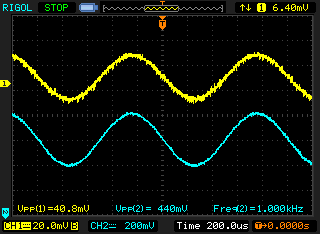
\includegraphics[width=\textwidth]{images/osc_exp5_vof_vacio.png}
        \caption{Tensión de salida en vacío ($V_o' = 440\mV_{pp}$).}
        \label{fig:osc_exp5_vof_vacio}
    \end{subfigure}
    \hfill
    \begin{subfigure}[b]{0.48\textwidth}
        \centering
        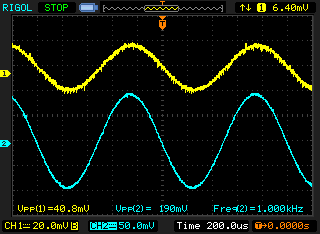
\includegraphics[width=\textwidth]{images/osc_exp5_vrl_realim_33ohm.png}
        \caption{Tensión sobre la carga de $33\ohm$ ($V_s' = 190\mV_{pp}$).}
        \label{fig:osc_exp5_vrl_realim_33ohm}
    \end{subfigure}
    \caption{Capturas de pantalla del osciloscopio en condición de lazo cerrado.}
    \label{fig:osc_exp5_lazo_cerrado_capturas}
\end{figure}

Los valores relevados en la experiencia se resumen en la Tabla~\ref{tab:exp5_lazo_cerrado}.

\begin{table}[!ht]
    \centering
    \resizebox{\textwidth}{!}{
    \begin{tabular}{|c|c|c|c|c|c|}
        \hline
        \textbf{Condición} & \textbf{$V_i$ [Vpp]} & \textbf{$V_o'$ (Vacío) [Vpp]} & \textbf{$V_s'$ (Carga $33\ohm$) [Vpp]} & \textbf{$R_{o,\text{calc}}'$ [$\ohm$]} & \textbf{$R_{o,\text{exp}}'$ [$\ohm$]} \\ \hline
        \textbf{Lazo Cerrado} & $40.8\mV$ & $440\mV$ & $190\mV$ & $34.7\ohm$ & $43.4\ohm$ \\ \hline
    \end{tabular}}
    \caption{Mediciones y comparación de la resistencia de salida a lazo cerrado.}
    \label{tab:exp5_lazo_cerrado}
\end{table}

\section{Experimento 6: Medición de la potencia eficaz máxima de salida}
Se analizó la máxima potencia eficaz antes del recorte (máxima excursión simétrica) en ambas configuraciones del amplificador. La potencia se calcula en base a la tensión eficaz sobre la carga respectiva ($R_L = R_o$ para lazo abierto, y $R_L = R_o'$ para lazo cerrado):
\begin{equation}
    P_{\text{máx}} = \frac{V_{\text{rms}}^2}{R_L} = \frac{V_{\text{pp}}^2}{8 \cdot R_L}
\end{equation}

El desarrollo de los cálculos para cada configuración es el siguiente:
\begin{enumerate}
    \item \textbf{Lazo Abierto} ($R_L = 560\ohm$ y $V_{o,\text{máx}} = 3.56\V_{pp}$, como se muestra en la Figura~\ref{fig:osc_exp5_vrlmax_560ohm}):
          \begin{equation}
              P_{\text{máx},\text{LA}} = \frac{(3.56\V_{pp})^2}{8 \cdot 560\ohm} = \approx 2.83\mW
          \end{equation}
    \item \textbf{Lazo Cerrado} ($R_L = 33\ohm$ y $V_{o,\text{máx}}' = 464\mV_{pp}$, como se muestra en la Figura~\ref{fig:osc_exp5_vrlmax_realim_33ohm}):
          \begin{equation}
              P_{\text{máx},\text{LC}} = \frac{(0.464\V_{pp})^2}{8 \cdot 33\ohm} = \approx 0.82\mW
          \end{equation}
\end{enumerate}

\begin{figure}[!ht]
    \centering
    \begin{subfigure}[b]{0.48\textwidth}
        \centering
        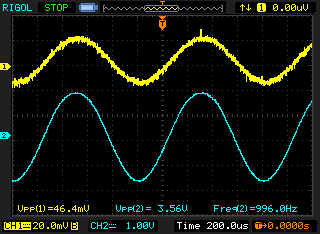
\includegraphics[width=\textwidth]{images/osc_exp5_vrlmax_560ohm.png}
        \caption{Máxima excursión a lazo abierto ($R_L = 560\ohm$, $V_{pp} = 3.56\V$).}
        \label{fig:osc_exp5_vrlmax_560ohm}
    \end{subfigure}
    \hfill
    \begin{subfigure}[b]{0.48\textwidth}
        \centering
        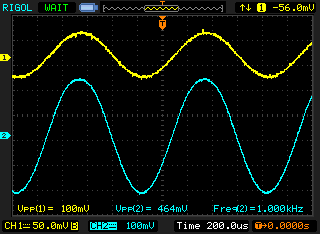
\includegraphics[width=\textwidth]{images/osc_exp5_vrlmax_realim_33ohm.png}
        \caption{Máxima excursión a lazo cerrado ($R_L = 33\ohm$, $V_{pp} = 464\mV$).}
        \label{fig:osc_exp5_vrlmax_realim_33ohm}
    \end{subfigure}
    \caption{Capturas de pantalla del osciloscopio para la medición de la máxima excursión simétrica.}
    \label{fig:osc_exp6_excursion_maxima}
\end{figure}

Los datos y el contraste de transferencia de potencia máxima se resumen en la Tabla~\ref{tab:exp6}.

\begin{table}[!ht]
    \centering
    \resizebox{\textwidth}{!}{
    \begin{tabular}{|l|c|c|c|}
        \hline
        \textbf{Configuración} & \textbf{Carga $R_L$ Ajustada} & \textbf{Tensión $V_{pp}$ [V]} & \textbf{Potencia $P_{\text{máx}}$ [mW]} \\ \hline
        \textbf{Lazo Abierto} & $560\ohm$ & $3.56\V$ & $2.83\mW$ \\ \hline
        \textbf{Lazo Cerrado} & $33\ohm$ & $0.464\V$ & $0.82\mW$ \\ \hline
    \end{tabular}}
    \caption{Comparación de la máxima transferencia de potencia eficaz.}
    \label{tab:exp6}
\end{table}

\section{Experimento 7: Ensayo de la respuesta en frecuencia (ancho de banda) del amplificador}
El relevamiento de la respuesta en frecuencia se realizó en vacío ($Js$ desconectado) mediante un barrido de frecuencia.
La señal de entrada se mantuvo constante y con nivel suficiente para máxima tensión de salida libre de distorsión
a la frecuencia de referencia ($1\kHz$). La ganancia relativa en decibeles se calcula como:
\begin{equation}
    \text{Ganancia Relativa [dB]} = 20 \cdot \log_{10} \left( \frac{V_o(f)}{V_o(1\kHz)} \right)
\end{equation}

Para determinar los valores de tensión correspondientes a las atenuaciones de
$-2\text{ dB}$ y $-3\text{ dB}$ respecto de la frecuencia de referencia
($1\kHz$), se utilizó la relación de atenuación en tensión:

\begin{equation}
    V_o(\text{dB}) = V_{\text{ref}} \cdot 10^{\frac{\text{dB}}{20}}
\end{equation}
Donde la tensión de referencia para máxima excursión a la frecuencia media de $1\kHz$ es:
\begin{itemize}
    \item Lazo abierto: $V_{\text{ref}} = V_o(1\kHz) = 7.2\V_{pp}$
    \item Lazo cerrado: $V_{\text{ref}}' = V_o'(1\kHz) = 8.16\V_{pp}$
\end{itemize}

De esta manera, los valores de tensión correspondientes a cada nivel de atenuación son:
\begin{itemize}
    \item \textbf{Lazo Abierto}:
          \begin{itemize}
              \item Tensión para $-2\text{ dB}$: $V_o(-2\dB) = 7.2\V \cdot 10^{\frac{-2}{20}} \approx 5.72\V_{pp}$
              \item Tensión para $-3\text{ dB}$: $V_o(-3\dB) = 7.2\V \cdot 10^{\frac{-3}{20}} \approx 5.10\V_{pp}$
          \end{itemize}
    \item \textbf{Lazo Cerrado}:
          \begin{itemize}
              \item Tensión para $-2\text{ dB}$: $V_o'(-2\dB) = 8.16\V \cdot 10^{\frac{-2}{20}} \approx 6.48\V_{pp}$
              \item Tensión para $-3\text{ dB}$: $V_o'(-3\dB) = 8.16\V \cdot 10^{\frac{-3}{20}} \approx 5.78\V_{pp}$
          \end{itemize}
\end{itemize}

Los valores de medición obtenidos mediante la experimentación en el laboratorio
se organizan en las Tablas~\ref{tab:exp7_abierto} y \ref{tab:exp7_cerrado}
respectivamente, donde se han incorporado dos valores intermedios a ambos lados
de la frecuencia media.

\begin{table}[!ht]
    \centering
    \resizebox{\textwidth}{!}{
    \begin{tabular}{|l|c|c|c|c|c|c|c|}
        \hline
        \textbf{Parámetro (L. A.)} & \textbf{$f_{\text{c-inf}}$ (-3 dB)} & \textbf{Frec. Intermedia (-2 dB)} & \textbf{Frec. Intermedia} & \textbf{Frec. Media (0 dB)} & \textbf{Frec. Intermedia} & \textbf{Frec. Intermedia (-2 dB)} & \textbf{$f_{\text{c-sup}}$ (-3 dB)} \\ \hline
        \textbf{Frecuencia [Hz]} & 54 $\Hz$ & 77 $\Hz$ & 500 $\Hz$ & $1000\Hz$ & 45k $\Hz$ & 72k $\Hz$ & 91.1k $\Hz$ \\ \hline
        \textbf{Salida [dB]} & $-3\text{dB}$ & $-2\text{dB}$ & $-0.3\text{dB}$ & $0\text{dB}$ & $-0.7\text{dB}$ & $-2\text{dB}$ & $-3\text{dB}$ \\ \hline
        \textbf{Tensión $V_o$ [V]} & $5.10\V$ & $5.72\V$ & $6.96\V$ & $7.20\V$ & $6.42\V$ & $5.72\V$ & $5.10\V$ \\ \hline
    \end{tabular}}
    \caption{Barrido de frecuencia del amplificador a lazo abierto.}
    \label{tab:exp7_abierto}
\end{table}

\begin{table}[!ht]
    \centering
    \resizebox{\textwidth}{!}{
    \begin{tabular}{|l|c|c|c|c|c|c|c|}
        \hline
        \textbf{Parámetro (L. C.)} & \textbf{$f_{\text{c-inf}}$ (-3 dB)} & \textbf{Frec. Intermedia (-2 dB)} & \textbf{Frec. Intermedia} & \textbf{Frec. Media (0 dB)} & \textbf{Frec. Intermedia} & \textbf{Frec. Intermedia (-2 dB)} & \textbf{$f_{\text{c-sup}}$ (-3 dB)} \\ \hline
        \textbf{Frecuencia [Hz]} & 10 $\Hz$ & 13 $\Hz$ & 500 $\Hz$ & $1000\Hz$ & 502.5k$\Hz$ & 1.34M $\Hz$ & 1.67M $\Hz$ \\ \hline
        \textbf{Salida [dB]} & $-3\text{ dB}$ & $-2\text{ dB}$ & $-0.086\text{ dB}$ & $0\text{ dB}$ & $-0.17\text{ dB}$ & $-2\text{ dB}$ & $-3\text{ dB}$ \\ \hline
        \textbf{Tensión $V_o'$ [V]} & $5.76\V$ & $6.48\V$ & $8.08\V$ & $8.16\V$ & $8.00\V$ & $6.52\V$ & $5.76\V$ \\ \hline
    \end{tabular}}
    \caption{Barrido de frecuencia del amplificador a lazo cerrado.}
    \label{tab:exp7_cerrado}
\end{table}
El ancho de banda determinado por barrido es:
\begin{itemize}
    \item $AB_{\text{L.A.}} = f_{\text{c-sup}} - f_{\text{c-inf}} = (91.1k-54)\Hz = 91.046k\Hz$
    \item $AB_{\text{L.C.}} = f_{\text{c-sup}} - f_{\text{c-inf}} = (1.67M-10)\Hz \approx 1.67M\Hz$
\end{itemize}

Se ha trazado los puntos relevados en el laboratorio y se han expuesto a modo
de comparación en la figura \ref{fig:respuesta_frecuencia_comparativa}.

\begin{figure}[!ht]
    \centering
    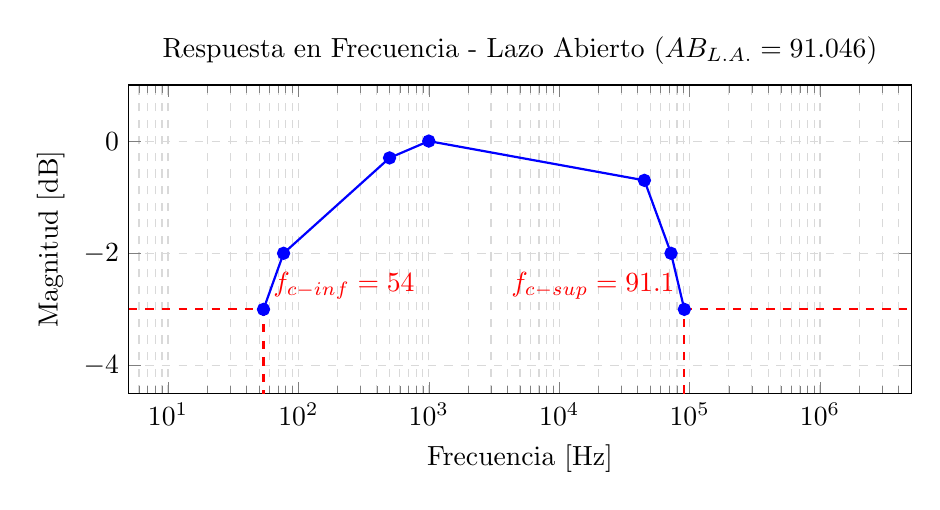
\begin{tikzpicture}
        \begin{semilogxaxis}[
            width=0.95\textwidth,
            height=5.5cm,
            xmin=5, xmax=5e6,
            ymin=-4.5, ymax=1,
            xlabel={Frecuencia [Hz]},
            ylabel={Magnitud [dB]},
            grid=both,
            grid style={dashed, gray!30},
            title={Respuesta en Frecuencia - Lazo Abierto ($AB_{\text{L.A.}} = 91.046\kHz$)},
            xticklabel style={/pgf/number format/fixed},
            title style={yshift=-0.5ex}
        ]
            \addplot[blue, thick, mark=*] coordinates {
                (54, -3)
                (77, -2)
                (500, -0.3)
                (1000, 0)
                (45000, -0.7)
                (72000, -2)
                (91100, -3)
            };
            % Dotted lines for -3dB cutoff points
            \draw[dashed, red, thick] (axis cs:5, -3) -- (axis cs:54, -3) -- (axis cs:54, -4.5);
            \draw[dashed, red, thick] (axis cs:91100, -4.5) -- (axis cs:91100, -3) -- (axis cs:5e6, -3);
            \node[red, above right] at (axis cs:54, -3) {$f_{\text{c-inf}}=54\Hz$};
            \node[red, above left] at (axis cs:91100, -3) {$f_{\text{c-sup}}=91.1\kHz$};
        \end{semilogxaxis}
    \end{tikzpicture}
    
    \vspace{0.3cm}
    
    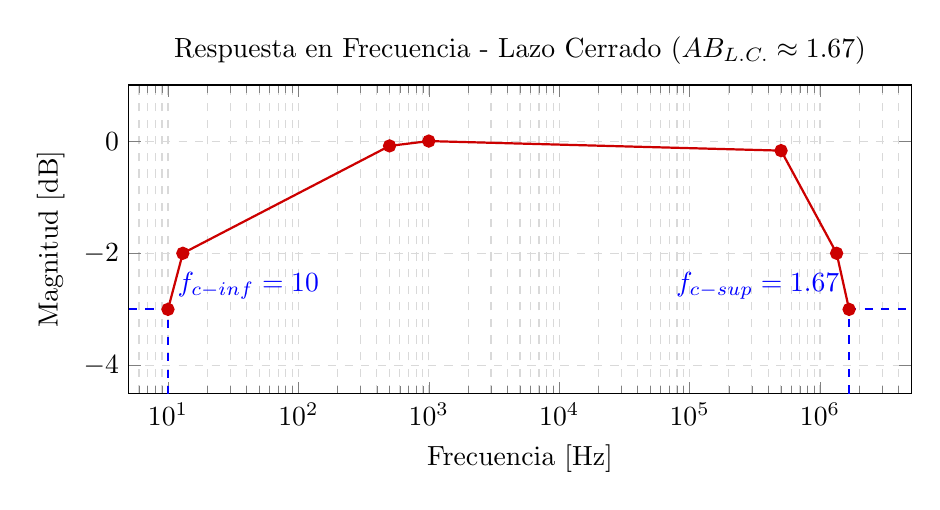
\begin{tikzpicture}
        \begin{semilogxaxis}[
            width=0.95\textwidth,
            height=5.5cm,
            xmin=5, xmax=5e6,
            ymin=-4.5, ymax=1,
            xlabel={Frecuencia [Hz]},
            ylabel={Magnitud [dB]},
            grid=both,
            grid style={dashed, gray!30},
            title={Respuesta en Frecuencia - Lazo Cerrado ($AB_{\text{L.C.}} \approx 1.67\MHz$)},
            xticklabel style={/pgf/number format/fixed},
            title style={yshift=-0.5ex}
        ]
            \addplot[red!80!black, thick, mark=*] coordinates {
                (10, -3)
                (13, -2)
                (500, -0.086)
                (1000, 0)
                (502500, -0.17)
                (1340000, -2)
                (1670000, -3)
            };
            % Dotted lines for -3dB cutoff points
            \draw[dashed, blue, thick] (axis cs:5, -3) -- (axis cs:10, -3) -- (axis cs:10, -4.5);
            \draw[dashed, blue, thick] (axis cs:1670000, -4.5) -- (axis cs:1670000, -3) -- (axis cs:5e6, -3);
            \node[blue, above right] at (axis cs:10, -3) {$f_{\text{c-inf}}=10\Hz$};
            \node[blue, above left] at (axis cs:1670000, -3) {$f_{\text{c-sup}}=1.67\MHz$};
        \end{semilogxaxis}
    \end{tikzpicture}
    \caption{Respuesta en frecuencia comparativa a lazo abierto y lazo cerrado.}
    \label{fig:respuesta_frecuencia_comparativa}
\end{figure}

\section{Experimento 8: Respuesta al escalón y estimación de ancho de banda mediante onda cuadrada}
Se aplicó una onda cuadrada de $1\kHz$ en la entrada del amplificador y se visualizó un único flanco de subida con ayuda del magnificador horizontal del osciloscopio ($X10$, debidamente calibrado). Se determinó el tiempo de crecimiento de salida ($t_{c,\text{medido}}$) medido entre el $10\%$ y el $90\%$ de la excursión total de amplitud.

Para obtener el tiempo de crecimiento propio del amplificador ($t_{c,\text{amplif}}$), se consideró el ancho de banda del osciloscopio ($AB_{\text{osc}} = 50\MHz$). El tiempo de crecimiento propio del osciloscopio ($t_{c,\text{osc}}$) y las correcciones correspondientes son:
\begin{equation}
    t_{c,\text{osc}} = \frac{0,35}{AB_{\text{osc}}} = \frac{0,35}{50\MHz} = 7\ns = 0,007\us
\end{equation}
\begin{equation}
    t_{c,\text{amplif}} = \sqrt{t_{c,\text{medido}}^2 - t_{c,\text{osc}}^2}
\end{equation}

El factor de proporcionalidad $k = 0,35$ en la relación $AB = k / t_c$ se
utiliza debido a que la caída de la curva de respuesta en frecuencia
(\textit{rolloff}) en la zona de alta frecuencia se comporta de manera suave y
sin sobreimpulso (característica de un sistema de primer orden con un único polo
dominante, donde la respuesta al escalón es una caída exponencial sin
oscilaciones). En cambio, si el amplificador presentara picos de resonancia en
su respuesta en frecuencia, existiría sobreimpulso y oscilaciones
en la respuesta al escalón en el dominio del tiempo, lo cual
requeriría emplear un factor de proporcionalidad mayor, típicamente de $k
\approx 0,4$. En la Figura~\ref{fig:comparacion_k_sobreimpulso} se ilustra esta
correspondencia teórica entre ambos dominios.

\begin{figure}[!ht]
    \centering
    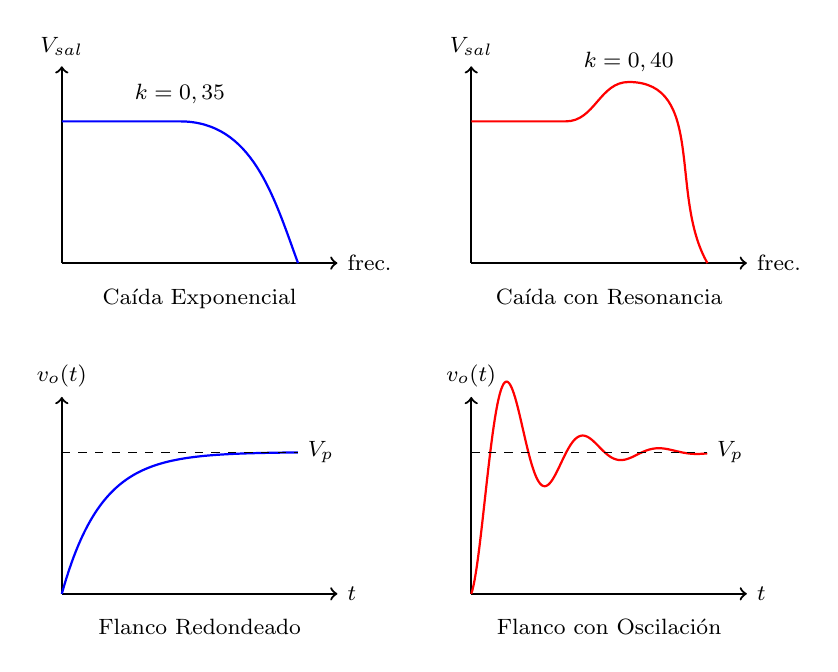
\begin{tikzpicture}
        % Left Column: Sin Sobreimpulso (k = 0.35)
        % Row 1: Frequency Domain
        \begin{scope}[shift={(0,4.2)}]
            \draw[->, thick] (0,0) -- (3.5,0) node[right] {\footnotesize frec.};
            \draw[->, thick] (0,0) -- (0,2.5) node[above] {\footnotesize $V_{\text{sal}}$};
            \draw[thick, blue] (0,1.8) -- (1.5,1.8) to[out=0,in=110] (3.0,0);
            \node[above] at (1.5,1.9) {\footnotesize $k = 0,35$};
            \node[below, align=center] at (1.75,-0.2) {\footnotesize Caída Exponencial};
        \end{scope}
        
        % Row 2: Time Domain (Step Response)
        \begin{scope}[shift={(0,0)}]
            \draw[->, thick] (0,0) -- (3.5,0) node[right] {\footnotesize $t$};
            \draw[->, thick] (0,0) -- (0,2.5) node[above] {\footnotesize $v_o(t)$};
            % Exponential rise
            \draw[thick, blue, domain=0:3, samples=100] plot (\x, {1.8*(1-exp(-\x*2.0))});
            \draw[dashed] (0,1.8) -- (3.0,1.8) node[right] {\footnotesize $V_{\text{p}}$};
            \node[below, align=center] at (1.75,-0.2) {\footnotesize Flanco Redondeado};
        \end{scope}

        % Right Column: Con Sobreimpulso (k = 0.4)
        % Row 1: Frequency Domain
        \begin{scope}[shift={(5.2,4.2)}]
            \draw[->, thick] (0,0) -- (3.5,0) node[right] {\footnotesize frec.};
            \draw[->, thick] (0,0) -- (0,2.5) node[above] {\footnotesize $V_{\text{sal}}$};
            % Peaking curve
            \draw[thick, red] (0,1.8) -- (1.2,1.8) to[out=0,in=180] (2.0,2.3) to[out=0,in=120] (3.0,0);
            \node[above] at (2.0,2.3) {\footnotesize $k = 0,40$};
            \node[below, align=center] at (1.75,-0.2) {\footnotesize Caída con Resonancia};
        \end{scope}
        
        % Row 2: Time Domain (Step Response with overshoot)
        \begin{scope}[shift={(5.2,0)}]
            \draw[->, thick] (0,0) -- (3.5,0) node[right] {\footnotesize $t$};
            \draw[->, thick] (0,0) -- (0,2.5) node[above] {\footnotesize $v_o(t)$};
            % Damped oscillation: 1.8 * (1 - exp(-1.5*x) * cos(5*x)) (roughly)
            \draw[thick, red, domain=0:3, samples=200] plot (\x, {1.8*(1 - exp(-1.5*\x)*cos(deg(6.5*\x)))});
            \draw[dashed] (0,1.8) -- (3.0,1.8) node[right] {\footnotesize $V_{\text{p}}$};
            \node[below, align=center] at (1.75,-0.2) {\footnotesize Flanco con Oscilación};
        \end{scope}
    \end{tikzpicture}
    \caption{Comparación de respuestas espectrales y temporales para distintos tipos de caída de la curva de ganancia ($k = 0,35$ vs. $k = 0,40$).}
    \label{fig:comparacion_k_sobreimpulso}
\end{figure}

El desarrollo de los cálculos y las estimaciones del ancho de banda ($AB = 0,35 / t_{c,\text{amplif}}$) para cada configuración son:
\begin{enumerate}
    \item \textbf{Lazo Abierto} ($t_{c,\text{medido, LA}} = 4.4\us$, como se muestra en la Figura~\ref{fig:osc_exp8_tr_la}):
          \begin{equation}
              t_{c,\text{amplif, LA}} = \sqrt{(4.4\us)^2 - (0.007\us)^2} \approx 4.4\us
          \end{equation}
          \begin{equation}
              AB_{\text{cuadrada, LA}} = \frac{0.35}{4.4\us} \approx 79.55\kHz
          \end{equation}
    \item \textbf{Lazo Cerrado} ($t_{c,\text{medido, LC}} = 190\ns$, como se muestra en la Figura~\ref{fig:osc_exp8_tr_lc}):
          \begin{equation}
              t_{c,\text{amplif, LC}} = \sqrt{(190\ns)^2 - (7\ns)^2} = \sqrt{36100 - 49}\ns \approx 189.87\ns = 0.1899\us
          \end{equation}
          \begin{equation}
              AB_{\text{cuadrada, LC}} = \frac{0.35}{189.87\ns} \approx 1843.36\kHz \approx 1.84\MHz
          \end{equation}
\end{enumerate}

\begin{figure}[!ht]
    \centering
    \begin{subfigure}[b]{0.48\textwidth}
        \centering
        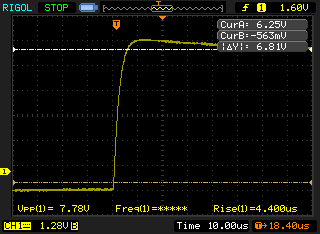
\includegraphics[width=\textwidth]{images/osc_exp8_tr_la.png}
        \caption{Tiempo de crecimiento a lazo abierto ($t_{c,\text{medido}} = 4.4\us$).}
        \label{fig:osc_exp8_tr_la}
    \end{subfigure}
    \hfill
    \begin{subfigure}[b]{0.48\textwidth}
        \centering
        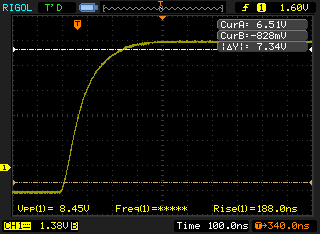
\includegraphics[width=\textwidth]{images/osc_exp8_tr_lc.png}
        \caption{Tiempo de crecimiento a lazo cerrado ($t_{c,\text{medido}} = 190\ns$).}
        \label{fig:osc_exp8_tr_lc}
    \end{subfigure}
    \caption{Capturas de pantalla del osciloscopio para la medición del tiempo de crecimiento ($t_c$).}
    \label{fig:osc_exp8_tiempos_crecimiento}
\end{figure}

Los resultados y el contraste entre el método temporal (onda cuadrada) y espectral (barrido senoidal de la sección anterior) se informan en la Tabla~\ref{tab:exp8}.

\begin{table}[!ht]
    \centering
    \resizebox{\textwidth}{!}{
    \begin{tabular}{|l|c|c|c|c|}
        \hline
        \textbf{Configuración} & \textbf{$t_{c,\text{medido}}$} & \textbf{$t_{c,\text{amplif}}$} & \textbf{$AB_{\text{cuadrada}}$} & \textbf{$AB_{\text{barrido}}$ (Exp 7)} \\ \hline
        \textbf{Lazo Abierto} & $4.4\us$ & $4.4\us$ & $79.55\kHz$ & $91.05\kHz$ \\ \hline
        \textbf{Lazo Cerrado} & $190\ns$ ($0.19\us$) & $189.87\ns$ ($0.19\us$) & $1.84\MHz$ ($1843.36\kHz$) & $1.67\MHz$ ($1670\kHz$) \\ \hline
    \end{tabular}}
    \caption{Comparación de anchos de banda medidos por método de onda cuadrada y barrido.}
    \label{tab:exp8}
\end{table}
